\subsection{模板方法模式(TemplateMethod)}

\subsubsection{模板方法模式简介}

模板方法模式是一种设计模式,它定义了一个算法的步骤,并允许子类为一个或多个步骤提供实现。这样,子类可以在不改变算法架构的情况下,重新定义算法的某些步骤。

模板方法模式的主要用途是让子类可以重新定义算法的某些步骤,而不改变算法的架构。这样,子类可以根据自己的需要,对算法进行定制,从而获得更高的灵活性和可扩展性。

例如,在银行业务处理中,可能需要对不同类型的账户进行处理,比如活期账户、定期账户和信用卡账户。使用模板方法模式,可以定义一个模板方法来处理这些账户,并允许子类为某些步骤提供实现,比如计算利息和扣除手续费。这样,子类就可以根据自己的需要,对算法进行定制,从而支持不同类型的账户。

模板方法模式的优点包括:
\begin{enumerate}
    \item 封装算法架构:模板方法模式可以封装算法的架构,让子类可以重新定义算法的某些步骤。
    \item 提高代码的复用性:通过抽象父类和模板方法,模板方法模式可以提高代码的复用性,减少重复的代码。
    \item 提高系统的灵活性:模板方法模式可以让子类对算法进行定制,从而提高系统的灵活性和可扩展性。
\end{enumerate}

模板方法模式的缺点包括:
\begin{enumerate}
    \item 可能会过度抽象:如果模板方法的接口过于抽象,可能会导致子类难以理解和使用它。
    \item 可能会增加系统的复杂度:如果模板方法过于复杂,可能会增加系统的复杂度,导致系统难以维护和扩展。
    \item 可能会掩盖子类的问题:如果子类存在问题,模板方法可能会掩盖这些问题,导致用户无法及时发现并解决问题。
\end{enumerate}

\subsubsection{模版方法模式在项目中的应用}

\begin{figure}[h]
    \centering
    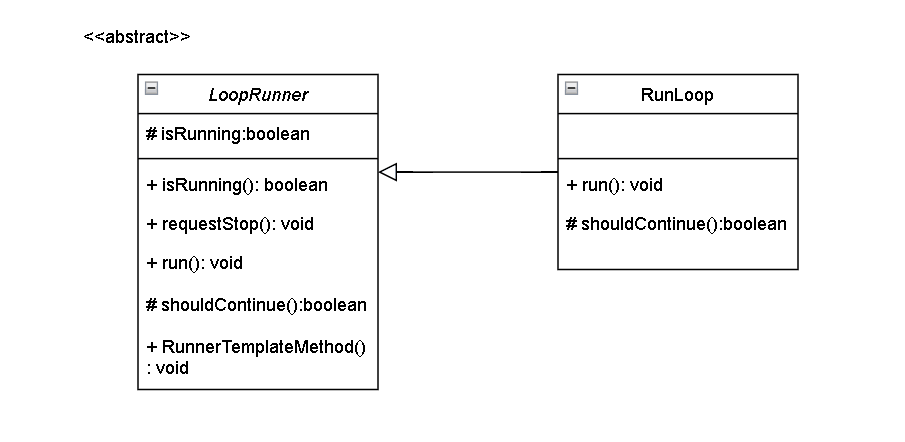
\includegraphics[width=0.9\textwidth]{figures/模板方法模式.png}
    \caption{模板方法模式在 Slow6502 中的类图}
\end{figure}

在本项目中,界面的事件循环就是基于模版方法模式构建的。在事件循环中,循环的大步骤被\lstinline{LoopRunner}定义,而\lstinline{RunLoop}通过继承\lstinline{LoopRunner}时实现其中的\lstinline{run()}方法实现在不改变算法架构的情况下,重新定义算法的某些步骤。
